\documentclass[sectionframe]{oxblue-beamer}

\usepackage{tikz}

\title{Introduction to Coding}
\author[Mape, R. N. R.]{Rixdon Niño R. Mape}
\institute{
    College of Science \\
    Computer Science and Information Technology Department \\
    Bicol University
}
\date{02 July 2024}

\begin{document}

\begin{frame}
\titlepage
\end{frame}

\section{Computer Abstraction}

\begin{frame}{What is a computer?}
A machine that receives, stores, transforms, and outputs data of all kinds, such as numbers, text, images, audio, graphics, etc.

\bigskip Categorized by size and performance.

\bigskip Used in various fields, such as education, business, entertainment, research, and more.
\end{frame}

\begin{frame}{Logical units of a computer}
\begin{itemize}
    \item Input unit
    \item Output unit
    \item Memory unit
    \item Arithmetic and logic unit (ALU)
    \item Central processing unit (CPU)
    \item Secondary storage unit
\end{itemize}
\end{frame}

\begin{frame}{Programming languages}
\begin{columns}
\begin{column}{0.3\textwidth}
    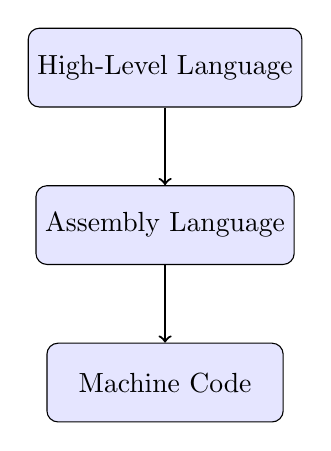
\begin{tikzpicture}[node distance=2cm]
        \tikzstyle{box} = [rectangle, rounded corners, minimum width=3cm, minimum height=1cm,text centered, draw=black, fill=blue!10]

        \node (high) [box] {High-Level Language};
        \node (assembly) [box, below of=high] {Assembly Language};
        \node (machine) [box, below of=assembly] {Machine Code};

        \draw [->,thick] (high) -- (assembly);
        \draw [->,thick] (assembly) -- (machine);
    \end{tikzpicture}
\end{column}
\begin{column}{0.6\textwidth}
    Programming in machine code is slow and error-prone. So, high-level languages were developed to make the process easier.

    \par\bigskip \begin{block}{Live Demo}
        Write, compile, and run a C program.
    \end{block}
\end{column}
\end{columns}
\end{frame}

\section{Software Development Method}

\begin{frame}{Define the problem}
State the problem clearly to gain a clear understanding of what is required for its solution. Eliminate unimportant details and focus on the core problem.

\par\bigskip \textbf{Sorting Robot Problem:}

Design an autonomous robot capable of sorting packages by size and destination in a logistics warehouse. The robot should operate with high accuracy and efficiency, reducing manual sorting tasks and improving overall processing speed.
\end{frame}

\begin{frame}{Analyze the problem}
Apply \textbf{computational thinking} to analyze complex problems and formulate effective solutions. These techniques can help you:

\begin{itemize}
    \item Break down the problem into smaller parts
    \item Identify patterns and relationships
    \item Focus on the essential details
    \item Develop a step-by-step plan
\end{itemize}
\end{frame}

\begin{frame}{Analyze the problem (cont'd)}
\textbf{Sorting Robot Problem}

\par\bigskip Break down the problem into smaller parts.

\par\bigskip How will the robot:
\begin{itemize}
    \item identify and localize packages?
    \item physically interact with packages?
    \item move around the warehouse?
    \item decide where to place each package?
    \item interact with other systems in the warehouse?
\end{itemize}
\end{frame}

\begin{frame}{Analyze the problem (cont'd)}
\textbf{Sorting Robot Problem}

\par\bigskip Identify patterns and relationships.

\par\bigskip \begin{itemize}
    \item Analyze historical sorting data to identify common package sizes, shapes, destinations, and sorting patterns.
    \item Learn from human sorters to observe their techniques, decision-making processes, and common challenges.
\end{itemize}

\end{frame}

\begin{frame}{Analyze the problem (cont'd)}
\textbf{Sorting Robot Problem}

\par\bigskip Focus on the essential details.

\par\bigskip Create simplified models for:
\begin{itemize}
    \item warehouse layout (e.g., grid-based map)
    \item package (e.g., size, weight, destination)
    \item robot capabilities (e.g., movement, sensors, manipulators)
\end{itemize}
\end{frame}

\begin{frame}{Design a solution}

Requires developing an \textbf{algorithm}, a replicable step-by-step process to accomplish a task.

\bigskip Use \textbf{top-down design} by first listing major steps, then breaking them down into smaller steps using \textbf{stepwise refinement}.
\end{frame}

\begin{frame}[fragile]{Design a solution (cont'd)}
\textbf{Sorting Robot Problem}

\bigskip Top-level algorithm:

\begin{verbatim}
1. Initialize the robot
2. Sort packages until none remain
3. Shutdown the robot
\end{verbatim}
\end{frame}

\begin{frame}[fragile]{Design a solution (cont'd)}
Refined algorithm:

\begin{verbatim}
1. Initialize:
    a. Load warehouse map
    b. Load package data
    c. Start communication with warehouse systems
2. While packages remain to be sorted:
    a. Scan the environment for packages
    b. Recognize package size and destination
    c. Determine where to place the package
    d. Navigate to the package
\end{verbatim}
\end{frame}

\begin{frame}[fragile]{Design a solution (cont'd)}
Refined algorithm (cont'd):

\begin{verbatim}
    e. Pick up the package
    f. Move to the designated location
    g. Place the package
    h. Notify the warehouse of the package's location
3. Shutdown:
    a. Report completion to the warehouse
    b. Safely power down the robot
\end{verbatim}
\end{frame}

\begin{frame}{Implement the solution}
Translate the algorithm into the programming language used by the robot.

\bigskip Write clean, readable, and maintainable code following established conventions and standards.

\bigskip Use Integrated Development Environments (IDEs), version control systems, and other tools to facilitate coding and collaboration.
\end{frame}

\begin{frame}{Test the program}
Use different testing methods to ensure the software works properly:

\begin{itemize}
    \item Unit testing (individual components)
    \item Integration testing (module interaction)
    \item System testing (simulation and real-world scenarios)
    \item Acceptance testing (stakeholder involvement)
\end{itemize}

\bigskip \begin{block}{Question}
    How would you test the sorting robot program?
\end{block}
\end{frame}

\begin{frame}{Refine the program}
\textbf{Refactor} the code by improving the internal structure of the code without changing its external behavior, making it easier to understand and modify.

\bigskip Write detailed \textbf{documentation} to help future developers understand the code and how to use or modify it.

\bigskip Gather \textbf{feedback} from users to identify areas for improvement and prioritize new features or fixes.
\end{frame}

\end{document}
